\begin{figure}[tbp]
\centering
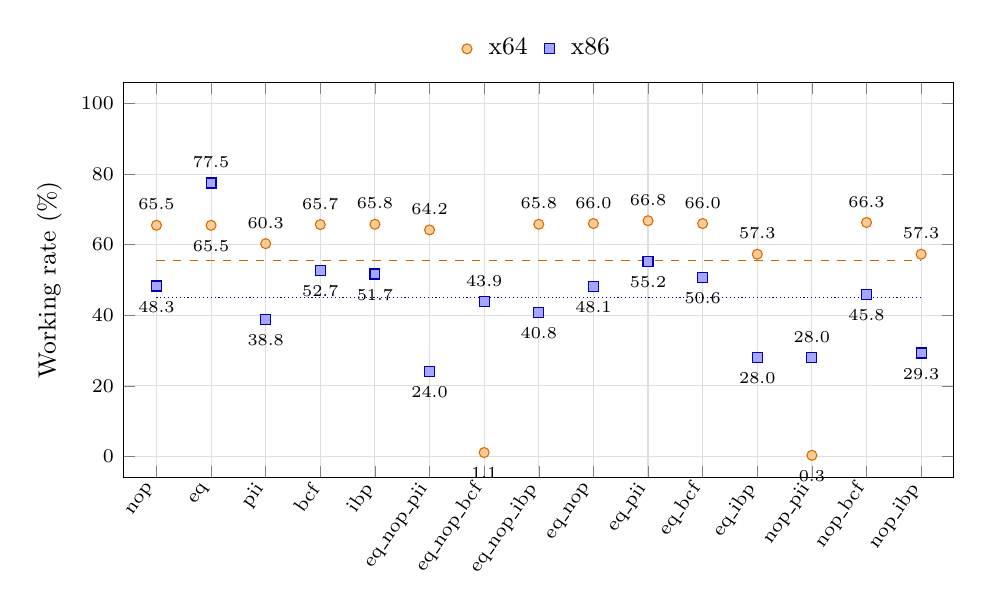
\begin{tikzpicture}
\begin{axis}[
width=\linewidth,height=6.6cm,
ylabel={Working rate (\%)},ymin=-6,ymax=106,xmin=-0.6,xmax=14.6,
xtick={0,...,14},
xticklabels={nop,eq,pii,bcf,ibp,eq\_nop\_pii,eq\_nop\_bcf,eq\_nop\_ibp,eq\_nop,eq\_pii,eq\_bcf,eq\_ibp,nop\_pii,nop\_bcf,nop\_ibp},
xticklabel style={rotate=55,anchor=east,font=\scriptsize},
yticklabel style={font=\scriptsize},label style={font=\small},
grid=major,grid style={gray!25},scaled y ticks=false,
legend style={at={(0.5,1.03)},anchor=south,legend columns=2,column sep=4pt,font=\small,draw=none},
clip=false,
]
\addplot[orange!80!black,dashed,no marks,forget plot] coordinates {(0,55.6) (14,55.6)};
\addplot[blue!65!black,densely dotted,no marks,forget plot] coordinates {(0,45.0) (14,45.0)};
\addplot[only marks,mark size=1.8pt,orange!85!black,mark=*,mark options={fill=orange!40}] coordinates {(0,65.5) (1,65.5) (2,60.3) (3,65.7) (4,65.8) (5,64.2) (6,1.1) (7,65.8) (8,66.0) (9,66.8) (10,66.0) (11,57.3) (12,0.3) (13,66.3) (14,57.3)};
\addlegendentry{x64}
\node[anchor=south,yshift=2pt,font=\fontsize{6}{7}\selectfont] at (axis cs:0,65.5) {65.5};
\node[anchor=north,yshift=-2pt,font=\fontsize{6}{7}\selectfont] at (axis cs:1,65.5) {65.5};
\node[anchor=south,yshift=2pt,font=\fontsize{6}{7}\selectfont] at (axis cs:2,60.3) {60.3};
\node[anchor=south,yshift=2pt,font=\fontsize{6}{7}\selectfont] at (axis cs:3,65.7) {65.7};
\node[anchor=south,yshift=2pt,font=\fontsize{6}{7}\selectfont] at (axis cs:4,65.8) {65.8};
\node[anchor=south,yshift=2pt,font=\fontsize{6}{7}\selectfont] at (axis cs:5,64.2) {64.2};
\node[anchor=north,yshift=-2pt,font=\fontsize{6}{7}\selectfont] at (axis cs:6,1.1) {1.1};
\node[anchor=south,yshift=2pt,font=\fontsize{6}{7}\selectfont] at (axis cs:7,65.8) {65.8};
\node[anchor=south,yshift=2pt,font=\fontsize{6}{7}\selectfont] at (axis cs:8,66.0) {66.0};
\node[anchor=south,yshift=2pt,font=\fontsize{6}{7}\selectfont] at (axis cs:9,66.8) {66.8};
\node[anchor=south,yshift=2pt,font=\fontsize{6}{7}\selectfont] at (axis cs:10,66.0) {66.0};
\node[anchor=south,yshift=2pt,font=\fontsize{6}{7}\selectfont] at (axis cs:11,57.3) {57.3};
\node[anchor=north,yshift=-2pt,font=\fontsize{6}{7}\selectfont] at (axis cs:12,0.3) {0.3};
\node[anchor=south,yshift=2pt,font=\fontsize{6}{7}\selectfont] at (axis cs:13,66.3) {66.3};
\node[anchor=south,yshift=2pt,font=\fontsize{6}{7}\selectfont] at (axis cs:14,57.3) {57.3};
\addplot[only marks,mark size=1.8pt,blue!70!black,mark=square*,mark options={fill=blue!35}] coordinates {(0,48.3) (1,77.5) (2,38.8) (3,52.7) (4,51.7) (5,24.0) (6,43.9) (7,40.8) (8,48.1) (9,55.2) (10,50.6) (11,28.0) (12,28.0) (13,45.8) (14,29.3)};
\addlegendentry{x86}
\node[anchor=north,yshift=-2pt,font=\fontsize{6}{7}\selectfont] at (axis cs:0,48.3) {48.3};
\node[anchor=south,yshift=2pt,font=\fontsize{6}{7}\selectfont] at (axis cs:1,77.5) {77.5};
\node[anchor=north,yshift=-2pt,font=\fontsize{6}{7}\selectfont] at (axis cs:2,38.8) {38.8};
\node[anchor=north,yshift=-2pt,font=\fontsize{6}{7}\selectfont] at (axis cs:3,52.7) {52.7};
\node[anchor=north,yshift=-2pt,font=\fontsize{6}{7}\selectfont] at (axis cs:4,51.7) {51.7};
\node[anchor=north,yshift=-2pt,font=\fontsize{6}{7}\selectfont] at (axis cs:5,24.0) {24.0};
\node[anchor=south,yshift=2pt,font=\fontsize{6}{7}\selectfont] at (axis cs:6,43.9) {43.9};
\node[anchor=north,yshift=-2pt,font=\fontsize{6}{7}\selectfont] at (axis cs:7,40.8) {40.8};
\node[anchor=north,yshift=-2pt,font=\fontsize{6}{7}\selectfont] at (axis cs:8,48.1) {48.1};
\node[anchor=north,yshift=-2pt,font=\fontsize{6}{7}\selectfont] at (axis cs:9,55.2) {55.2};
\node[anchor=north,yshift=-2pt,font=\fontsize{6}{7}\selectfont] at (axis cs:10,50.6) {50.6};
\node[anchor=north,yshift=-2pt,font=\fontsize{6}{7}\selectfont] at (axis cs:11,28.0) {28.0};
\node[anchor=south,yshift=2pt,font=\fontsize{6}{7}\selectfont] at (axis cs:12,28.0) {28.0};
\node[anchor=north,yshift=-2pt,font=\fontsize{6}{7}\selectfont] at (axis cs:13,45.8) {45.8};
\node[anchor=north,yshift=-2pt,font=\fontsize{6}{7}\selectfont] at (axis cs:14,29.3) {29.3};
\end{axis}
\end{tikzpicture}
\Description{Variants passing the published functional checks. Dashed reference lines show the reported architecture averages (x64: 55.6\%; x86: 45.0\%). Orange circles identify x64 and blue squares identify x86.}
\caption{Variants passing the published functional checks. Dashed reference lines show the reported architecture averages (x64: 55.6\%; x86: 45.0\%). Data from Fig.~3 of~\cite{zone_secrypt_2026}; redrawn for the present format.}
\label{fig:working_rate}
\end{figure}
